\section{Relativistische Quantenmechanik}
\subsection{Die Dirac-Gleichung}
NR QM:
	\begin{align*}
		H &= \frac{p^2}{2m} 
		& \vec{p} &\mapsto \hat{\vec{p}} = -i \hbar \vec{\nabla} \\
		& & E &\mapsto H = i \hbar \frac{\partial}{\partial t} \\
		i \hbar \frac{\partial}{\partial t} \ket{\psi} 
		&= \frac{\hat{p}^2}{2m} \ket{\psi} 
	\end{align*}
Spezielle Relativitätstheorie:
	\begin{align*}
		H^2 &= p^2 c^2 + m^2 c^4 
		&\Rightarrow H &= \sqrt{p^2c^2 +m^2 c^4} 
		= mc^2\left(1 + \frac{\vec{p}^2}{2m} - \frac{(\vec{p}^2)^2}{8 m^4 c^4} + \ldots\right)
	\end{align*}
Relativistische Schrödinger Gleichung (?):
	\begin{align*}
		i \hbar \frac{\partial}{\partial t} \ket{\psi} 
		= \sqrt{p^2c^2 +m^2 c^4} \ket{\psi}
	\end{align*}
Ortsraum:
	\begin{align*}
		i \hbar \frac{\partial}{\partial t} \ket{\psi} 
		= mc^2 \left(1 - \frac{\vec{\hbar^2}}{2mc^2}\vec{\nabla}^2 - \frac{\hbar^2(\vec{\nabla}^2)^2}{8 m^4 c^4}\right)
	\end{align*}
	\begin{enumerate}
		\item unsymmetrisch im Raum und Zeit (nicht forminvariant unter Lorentz-Transformation)
		\item Hohe Ableitungen
	\end{enumerate}
Zwei Möglichkeiten der relativen Verallgemeinerung der (freien) Schrödingergleichung 
\marginpar{?? punkt 2 kam nie vor}
	\begin{align*}
		H^2 \ket{\psi} &= (c^2 \hat{p}^2 + m^2 c^4) \ket{\psi} \\
		-\hbar^2 \frac{\partial^2 \psi}{\partial t^2}
		&= (-\hbar^2 c^2 \vec{\nabla}^2 + m^2 c^4) \psi (\vec{r} , t) \\
		&\Rightarrow
		\boxed{
			\left(
			\frac{1}{c^2} \frac{\partial^2 \psi}{\partial t^2} - \vec{\nabla}^2 
			+ \left(\frac{mc}{\hbar}\right)^2
			\right)
			\psi (\vec{r} , t) = 0
		}
	\end{align*} 
Klein-Gordon-Gleichung, und $\frac{1}{c^2} \frac{\partial^2 \psi}{\partial t^2} - \vec{\nabla}^2 = \Box$ d'Alembertoperator.

Kein ``Spin'' Möglich für skalare Teilchen

Spin $=0$: Higgs, Pionen, $\alpha-$Teilchen etc.
\\
Dirac: erste Ableitun in $t \Rightarrow$ sollte linear in $p_x, p_y, p_z$ sein, damit forminvariant unter Lorentz-Transformation.

Ansatz:
	\begin{align*}
		H^2 &= p^2 c^2 + m^2 c^4 = c^2 (\vec{\alpha} \cdot \vec{p} + \beta m c)^2\\
		&= c^2 
		\left[
			\alpha_x^2 p_x^2 + \alpha_y^2 p_y^2 +\alpha_z^2 p_z^2
			+ \beta^2m^2c^2 + \alpha_x \beta p_x m c + \beta \alpha_x p_x mc \right.\\
			&\left.\vphantom{\alpha_x^2 p_x^2} + \{\alpha_y, \beta\} p_y mc + \{\alpha_z \beta \} p_z mc 
			+ \{\alpha_x, \alpha_y\} p_x p_y + \{\alpha_y, \alpha_z\} p_y p_z
			+\{\alpha_z, \alpha_x\}p_z p_x
 		\right]
	\end{align*}
Koeffizientenvergleich:
	\begin{align*}
		\alpha_x^2 &= \alpha_y^2 = \alpha_z^2 = 1 = \beta^2
		& &\boxed{\{\alpha_i, \beta \} = 0}\\
		& & &\{\alpha_i, \beta \} = 0 \text{ für } i \neq j \\
		&\Rightarrow \boxed{\{\alpha_i, \beta \} = 2 \delta_{ij}}
	\end{align*}
$\Rightarrow \alpha_i, \beta$ sind keine Zahlen. (vllt Matrizen?)
	\begin{align*}
		\alpha_i &= \alpha_i^\dagger ,&
		\beta &= \beta^\dagger ,& 
		\text{weil } H &= H^\dagger \\
		\text{EW }: \alpha_i^2 &= \mathds{1} ,&
		\beta^2 &= \mathds{1} 
		&\Rightarrow \mathrm{ EW } &\in \{\pm 1\}  
	\end{align*}
	\begin{align*}
		\mathrm{Sp}(\alpha_x) = \mathrm{Sp}(\alpha_x\alpha_y^2) 
		= \mathrm{Sp} (\alpha_y \alpha_x \alpha_y) 
		= - \mathrm{Sp}(\alpha_x \alpha_y^2) = -\mathrm{Sp}(\alpha_x) = 0
	\end{align*}
$\alpha_i, \beta$ sind spurlose hermitesche Matrizen mit EW $\pm 1$
	\begin{align*}
		\text{spurlos } \Rightarrow \# (\mathrm{EW } = + 1)
		= \# (\mathrm{EW } = - 1) \Rightarrow \text{ Dimension }d\text{ gerade}
	\end{align*}
Bei $d=2$ haben wir die Paulimatrizen: Basis über $\mathds{R}$ aller spurlosen hermiteschen $2 \times 2$ Matrizen.
	\begin{align*}
		\sigma_x &=
		\begin{pmatrix}
		0 & 1 \\
		1 & 0
		\end{pmatrix}&
		\sigma_y &=
		\begin{pmatrix}
		0 & -i \\
		i & 0
		\end{pmatrix}&
		\sigma_z &= 
		\begin{pmatrix}
		1 & 0 \\
		0 & -1
		\end{pmatrix} \\
		\{\sigma_i, \sigma_j\} &= 2 \delta_{ij} 
		&\text{Nehme } \sigma_0 &=
		\begin{pmatrix}
		1 & 0 \\
		0 & 1
		\end{pmatrix}
		= \mathds{1}_2 \text{ hinzu} 
	\end{align*}
Problem: $\mathds{1}_2$ ist nicht spurlos

Kleinste mögliche Dimension ist $d = 4$
\\
Dirac- $\alpha,\beta$ Matrizen:
	\begin{align*}
		\vec{\alpha} &=
		\begin{pmatrix}
		0 & \vec{\sigma} \\
		\vec{\sigma} & 0
		\end{pmatrix} 
		& 4 \times 4 \text{ Matrix Beispiel: }
		\alpha_z &=
		\begin{pmatrix}
		0 & \sigma_z \\
		\sigma_z & 0
		\end{pmatrix}
		=
		\begin{pmatrix}
		0 & 0 & 1 & 0 \\
		0 & 0 & 0 & -1 \\
		1 & 0 & 0 & 0\\
		0 & -1 & 0 & 0
		\end{pmatrix} \\
		\beta &=
		\begin{pmatrix}
		\mathds{1}_2 & 0 \\
		0 & \mathds{1}_2
		\end{pmatrix}
	\end{align*}
$\vec{\alpha}, \beta$ sind nicht eindeutig festgelegt, da auch $\vec{\alpha}', \beta'$ mit 
$\alpha_i' = \U^\dagger \alpha_i \U,~ \beta' = \U^\dagger \beta \U$ ($\U$ unitäre Matrix) obige Bedingungen erfüllen.
	\begin{align*}
		-i\hbar \frac{\partial}{\partial t} \ket{\psi}
		&= \left(\vec{\alpha} c \vec{p} + \beta m c^2\right) \ket{\psi} \\
		\text{Ortsraum } i\hbar \frac{\partial \psi (\vec{r}, t)}{\partial t}
		&= \left(-i\hbar c \vec{\alpha} \vec{\nabla} + \beta m c^2\right) \psi (\vec{r}, t)
	\end{align*}
DGL 1.Ordnung in $\frac{\partial}{\partial t}$ und $\frac{\partial}{\partial x}, \frac{\partial}{\partial y}, \frac{\partial}{\partial z}$ aber $\psi (\vec{r}, t)$ hat 4 Komponenten.

$\Rightarrow$ Lorentz-Spinor
\\
 \marginpar{30.11.2015}
% Wdh
%	\begin{align*}
%		i \hbar \frac{\partial}{\partial t} \ket{\psi} &=
%		\left(c \vec{\alpha} \cdot \vec{p} + \beta m c^2\right) \ket{\psi}
%	\end{align*}
Dirac-Spinor (auch Lorentz-Spinor)
	\begin{align*}
		\psi (\vec{r}, t) &=
		\begin{pmatrix}
		\psi_1 (\vec{r}, t) \\
		\psi_2 (\vec{r}, t) \\
		\psi_3 (\vec{r}, t) \\
		\psi_4 (\vec{r}, t)
		\end{pmatrix} &
		\braket{\psi | \psi}
		&= \int \diff^3 r 
		\overbrace{\psi^\dagger (\vec{r}, t) \psi (\vec{r}, t)}^{\mathclap{\rho (\vec{r}, t)}} 
		= const.
	\end{align*}
Denn $H$ ist selbstadjungiert. 

$\leadsto$ Wahrscheinlichkeitsinterpretation mit $\braket{\psi | \psi} = 1$ ist möglich.
\\
Definiere Wahrscheinlichkeitsdichte $\rho (\vec{r}, t) = \psi^\dagger (\vec{r}, t) \psi (\vec{r}, t)$
	\begin{align*}
		\frac{\partial \rho}{\partial t} &= 
		\frac{\partial \psi^\dagger}{\partial t} \cdot \psi + \psi^\dagger \frac{\partial \psi}{\partial t} 
		= \left(
			\frac{\beta m c^2}{i \hbar} - \frac{\beta m c^2}{i \hbar} 
		\right)
		\psi^\dagger \psi - c\psi^\dagger \vec{\alpha} \vec{\nabla} \psi 
		- c \vec{\nabla} (\psi^\dagger \vec{\alpha}) \psi \\
		&= -c \vec{\nabla} (\psi^\dagger \vec{\alpha} \psi) 
	\end{align*}
	\begin{empheq}[box = \boxed]{align*}
		\Rightarrow \frac{\partial \rho}{\partial t} + \vec{\nabla} \vec{j} = 0&
		& &\text{mit } \vec{j} = c \psi^\dagger \alpha \psi \\
		\text{ Kontinuiätsgleichung}& & &\text{Wahrscheinlichkeitsstromdichte}
	\end{empheq}
	\begin{align*}
		4 \text{ Vektoren } (X^\mu) &= (X^0, \vec{X})
		& (X_\mu) &= (\eta_{\mu\nu} X^\nu) = (X^0, -\vec{X}) \\
		\eta_{\mu\nu} &=
		\begin{pmatrix}
			1 & 0 & 0 & 0 \\
			0 & -1 & 0 & 0 \\
			0 & 0 & -1 & 0 \\
			0 & 0 & 0 &-1
		\end{pmatrix} &
		\vec{X} &= 
		\begin{pmatrix}
		X^1 \\
		X^2 \\
		X^3 \\
		X^4 
		\end{pmatrix} \\
		\frac{\partial}{\partial X^\mu} X^\nu 
		&= \partial_\mu^\nu 
		\leadsto \partial_\mu = \frac{\partial}{\partial X^\mu}
	\end{align*}
(aus unten oben wird oben unten) $\partial_\mu X^\nu = \partial_\mu^\nu$
	\begin{align*}
		\left(\partial_\mu\right) 
		&= \left(\frac{\partial}{\partial X^\mu}\right)
		= (\partial_0, \vec{\nabla}) &
		(\partial^\mu) &=
		\left(\frac{\partial}{\partial X_\mu}\right)
		= (\partial^0, -\vec{\nabla}) \\
		\partial_0 &= \frac{\partial}{\partial X^0} = \frac{1}{c} \frac{\partial}{\partial t}
		& X^0 &= ct \\
		\vec{p} &= -i\hbar \vec{\nabla} ,&
		E &= i \hbar \frac{\partial}{\partial t} = i \hbar c \frac{\partial}{\partial X^0} 
	\end{align*}
4-Impuls $(p^\mu) = (E/c, \vec{p})$
	\begin{align*}
		p_\mu p^\mu &= \frac{E^2}{c^2} - \vec{p}^2 = m^2 c^2,&
		\text{denn } E^2 &= m^2 c^4 + \vec{p}^2 c^2 \\
		(p_\mu) &= \left(\frac{E}{c}, -\vec{p}\right) = i\hbar (\partial_0, \vec{\nabla})
	\end{align*}
	\begin{align*}
		0 &= \left(
			-i \hbar c \vec{\alpha}_i \vec{\nabla} - i\hbar \frac{\partial}{\partial t}
			+ \beta m c^2
		\right) \psi(\vec{r}, t) & 
		&\left.\vphantom{\left(\frac{\partial}{\partial t}\right)}\right| \cdot (-\beta) \\
		0 &= \left[
			i \hbar \left(\beta \frac{\partial}{\partial X^0} \beta \vec{\alpha} \vec{\nabla}\right)
			- mc
		\right] \psi (\vec{r}, t) \\
		\gamma^0 &= \beta ~,~~ \gamma^i =\beta \alpha^i \\
		0 &= \left(i \hbar 
			\left(\gamma^0 \frac{\partial}{\partial X^0} + \vec{\gamma} \cdot \vec{\nabla}\right)
			- mc
		\right) \psi (\vec{r}, t) 
	\end{align*}
	\begin{empheq}[box = \boxed]{align*}
		(i\hbar \gamma^\mu \partial_\mu - mc) \psi(\vec{r}, t) &= 0 \\
		\text{oder } (\gamma^\mu p_\mu - mc) \ket{\psi} &= 0
	\end{empheq}
Dirac Gleichung
	
Offensichtlich ist dies forminvariant unter Lorentz-Transformationen (relativistisch kovariant)
	\begin{align*}
		\gamma^0 &= \beta =
		\begin{pmatrix}
			\mathds{1} & 0 \\
			0 & -\mathds{1}
		\end{pmatrix}
		& \beta \cdot \alpha^i &= -\alpha^i \beta &
		&\{\alpha^i, \beta \} = 0 \\
		\vec{\gamma} &= \beta \vec{\alpha} =
		\begin{pmatrix}
			0 & \vec{\sigma} \\
			\vec{\sigma} & 0
		\end{pmatrix} &
		(\gamma^i)^\dagger &= (\beta \alpha^i)^\dagger
		= (\alpha^i)^\dagger \beta^\dagger \\
		& & &= \alpha^i \beta = -\beta \alpha^i = -\gamma^i
		& &\text{ (anti-hermitesch)} \\
		\gamma^0 &= (\gamma^0)^\dagger 
		& \boxed{(\gamma^\mu)^\dagger = \gamma^0 \gamma^\mu \gamma^0}&
	\end{align*}
	\begin{align*}
		\{\gamma^\mu, \gamma^\nu\} &= 2 g^{\mu \nu} = \mathds{1}_4\\
		\{\gamma^i, \gamma^j\} &=
		\{\beta \alpha^i, \beta \alpha^j\}
		= - \beta^2 \{\alpha^i, \alpha^j\} = -2 \delta^{ij} \mathds{1}\\
		\left[
			(\gamma^\mu p_\mu - m c) \psi
		\right]^\dagger &= 0 
		= \psi^\dagger (\gamma^{\mu \dagger} p_\mu - mc) \\
		&= \psi^\dagger \left(
			\gamma^0 \gamma^\mu p_\mu \gamma^0 - \gamma^0 mc \gamma^0
		\right) \\
		0 &= \psi^\dagger \gamma^0 (\gamma^\mu p_\mu - mc) \\
		\overline{\psi} \coloneqq \psi^\dagger \gamma^0
	\end{align*}
Wahrscheinlichkeitsstromdichte (0-Komponente):
	\begin{align*}
		j^0 &= c \rho = c \psi^\dagger \psi = c \overline{\psi} \gamma^0 \psi \\
		\frac{\partial \rho}{\partial t}
		&= \partial_0 j^0 = -\vec{\nabla} \psi^\dagger \vec{\alpha} \psi 
		= - \partial_i \overline{\psi}
		\underbrace{\gamma^0 \alpha^i}_{\mathclap{\beta \alpha^i = \gamma^i}} \psi \\
		\Rightarrow \partial_\mu 
		\underbrace{\overline{\psi} \gamma^\mu \psi}_{\mathclap{\text{Der 4-Strom }j^\mu \text{ ist erhalten}}} &= 0 ~~\text{(Kontinuitätsgleichung)}
	\end{align*}
	\begin{align*}
		\psi &=
		\begin{pmatrix}
			\psi_1 \\
			\psi_2 \\
			\psi_3 \\
			\psi_4
		\end{pmatrix}
		&\Rightarrow \overline{\psi} &=
		(\psi_1^*, \psi_2^*, -\psi_3^*, -\psi_4^*) 
	\end{align*}
Ansatz ebene Welle:
	\begin{align*}
		\psi (\vec{r}, t) &=
		u(\vec{k}) e^{i(\vec{k}\vec{r} - \omega(\vec{k}) t)} \\
		&= u(\vec{k}) e^{ik.x} 
		& &k. x= k_\mu X^\mu \\
		\vec{X} &= \vec{r} ,& X^0 &= ct,& k^0 &= \frac{\omega}{c} \\
		u &=
		\begin{pmatrix}
			u_1 \\
			u_2 \\
			u_3 \\
			u_4
		\end{pmatrix}
		~ \text{ Dirac Spinor}
	\end{align*}
	\begin{align*}
		\left(i \hbar \gamma^\mu \partial_\mu - mc\right)
		\psi(\vec{r}, t) &= 0 \\
		\text{ist OK für } p_\mu p^\mu &= m^2 c^2 \\
		\Rightarrow (\gamma^\mu p_\mu - mc) u \left(\vec{k} = \frac{\vec{p}}{\hbar}\right) &= 0 
	\end{align*}
Lösung für $\vec{p} = \vec{0}$ mit 
$ \gamma^0\begin{pmatrix}
1 & & \\
& 1 && \\
&& -1 & \\
&&& -1 
\end{pmatrix}$
	\begin{align*}
		(\gamma^0 p_0 - mc) u = 0 \Rightarrow
		(E-mc^2) u_1 &= 0 \\
		(E-mc^2) u_2 &= 0 \\
		(-E-mc^2) u_3 &= 0 \\
		(-E-mc^2) u_4 &= 0 \\
	\end{align*}
	\begin{align*}
		\Rightarrow 4 \text{ Lösungen }: 
		E &= mc^2 ,& u^{(1)} &= (1, 0 ,0 ,0)^t &\text{ oder } 
		u^{(2)} &= (0,1,0,0)^t \\
		E &= -mc^2 ,& u^{(3)} &= (0, 0, 1, 0)^t &\text{ oder }
		u^{(4)} &= (0,0,0,1)^t
	\end{align*}
Beliebiger Impuls:
	\begin{align*}
	u &= 
		\begin{pmatrix}
			\phi \\
			\chi
		\end{pmatrix} &
	\phi &= 
		\begin{pmatrix}
		\phi_1 \\
		\phi_2
		\end{pmatrix} &
	\chi &= 
		\begin{pmatrix}
		\chi_1 \\
		\chi_2
		\end{pmatrix}
	\end{align*}
	\begin{align*}
		\left( \gamma^\mu p_\mu - mc\right) u
		&=\left[
			\gamma^0 \left(
				\mathds{1} p_0 +
					\begin{pmatrix}
						0 & \vec{\sigma} \\
						\vec{\sigma} & 0
					\end{pmatrix} \vec{p}
				\right)
			-mc \mathds{1}
		\right]
		\begin{pmatrix}
			\phi \\
			\chi
		\end{pmatrix} \\
		&= \begin{pmatrix}
			(p_0 -mc) \phi - (\vec{p} ~\vec{\sigma}) \chi \\
			(-p_0 -mc) \chi - (\vec{p} ~\vec{\sigma}) \phi
		\end{pmatrix}
		= \vec{0}
	\end{align*}
	\begin{align*}
		\text{2.Zeile: }
		\chi &= \frac{- \vec{p}~\vec{\sigma}}{p_0 +mc} \phi 
		& (\vec{A}\vec{\sigma})(\vec{B}\vec{\sigma}) &=
		\vec{A}\vec{B}+ i \vec{\sigma} (\vec{A} \times \vec{B}) \\
		\text{1.Zeile: } 
		\phi &= - \frac{\vec{p}~\vec{\sigma}}{p_0 - mc} \chi \\
		&= \frac{(\vec{p}~\vec{\sigma})(\vec{p}~\vec{\sigma})}{p_0^2-m^2c^2} \phi \\
		&= \frac{\vec{p}^2}{\vec{p}^2}\phi = \phi \checkmark
	\end{align*}
Also $\phi$ und $\chi$ nicht linear unabhängig.
	\begin{align*}
		\boxed{E^2 = \vec{p}^2c^2 + m^2 c^4}
	\end{align*}
$\Rightarrow$ Es existieren ebene Wellen als Lösungen der Dirac Gleichung, wobei $\phi$ oder $\chi$ frei gewählt werden kann.

2 Fälle(analog zum $\vec{p}= \vec{0}$ Fall)
	\begin{enumerate}[1.]
		\item $E= \sqrt{m^2c^4 + \vec{p}^2 c^2}$
		\begin{align*}
			\psi (x) &= u(\vec{k}) e^{-ik.x} \\
			\phi^{(1)} &= 
			\begin{pmatrix}
			1 \\ 0
			\end{pmatrix}
			&\Rightarrow 
			\chi^{(1)} &= \frac{\vec{p}~\vec{\sigma}}{p_0 + mc}
			\begin{pmatrix}
			1 \\ 0
			\end{pmatrix}
			= \frac{c}{E + mc^2}
			\begin{pmatrix}
			p_3 \\ p_1 + ip_2
			\end{pmatrix} 
			\\
			\phi^{(2)} &= 
			\begin{pmatrix}
			0 \\ 1
			\end{pmatrix}
			&\Rightarrow 
			\chi^{(2)} &= \frac{\vec{p}~\vec{\sigma}}{p_0 + mc}
			\begin{pmatrix}
			0 \\ 1
			\end{pmatrix}
			= \frac{c}{E + mc^2}
			\begin{pmatrix}
			p_1 - ip_2 \\ -p_3
			\end{pmatrix}
		\end{align*}
	Nicht relativistischer Grenzfall:
		\begin{align*}
			E &= mc^2 + E' &\text{mit } E' &\ll mc^2 \\
			E' &\approx \frac{\vec{p}^2}{2m} &
			\left|\chi^{(i)} \right| &\ll \left|\phi^{(i)} \right| \\
			\phi &: \text{``große Komponenten''} ,& \chi &: \text{``kleine Komponenten''}
		\end{align*}
	\item $E=-\sqrt{m^2c^4 + \vec{p}^2 c^2}$
		\begin{align*}
			\psi &= u(\vec{k}) e^{-ik.x} \\
			\Rightarrow 
			\chi^{(3)} &= 
			\begin{pmatrix}
			1 \\ 0
			\end{pmatrix}
			&\Rightarrow 
			\phi^{(3)} &= \frac{\vec{p}~\vec{\sigma}}{-p_0 + mc}
			\begin{pmatrix}
			1 \\ 0
			\end{pmatrix}
			= \frac{c}{|E| + mc^2}
			\begin{pmatrix}
			p_3 \\ p_1 + ip_2
			\end{pmatrix} 
			\\
			\chi^{(4)} &= 
			\begin{pmatrix}
			0 \\ 1
			\end{pmatrix}
			&\Rightarrow 
			\phi^{(4)} &= \frac{\vec{p}~\vec{\sigma}}{-p_0 + mc}
			\begin{pmatrix}
			0 \\ 1
			\end{pmatrix}
			= \frac{c}{|E| + mc^2}
			\begin{pmatrix}
			p_1 - ip_2 \\ -p_3
			\end{pmatrix}
			\\
			\phi &: \text{``kleine Komponenten''} ,& \chi &: \text{``große Komponenten''}
		\end{align*}
	im nicht relativistischen Grenzfall.
	\end{enumerate}
Wdh.: Lösung \marginpar{03.12.2015}
der ``freien'' Dirac-Gleichung 
	\begin{align*}
		\psi &= u(\vec{k}) e^{-ik.x} ,&
		k^2 &= k_\mu k^\mu = \frac{m^2 c^2}{\hbar^2} \\
		u &=
		\begin{pmatrix}
		\phi \\
		\chi
		\end{pmatrix}
		\text{und } \phi, \chi \text{ sind Pauli-Spinoren}		
	\end{align*}
Lösung mit $E > 0 \leadsto \phi$ große Kompontenten 
\\
Lösung mit $E < 0 \leadsto \chi$ große Kompontenten

Interpretation:
	\begin{align*}
		E>0 &: \text{ Elektron} \\
		E<0 &: \text{ Positron mit } E>0 \text{ (Antiteilchen)}
	\end{align*}
Es zeigt sich, dass $m(\text{Elektron}) = m{(Positron)}$, 
\\aber Ladung $q(\text{Elektron}) = -q(\text{Positron}) = -e$
\newpage
Dirac: ``Dirac''-See
	\begin{figure*} [h]
		\begin{center}
			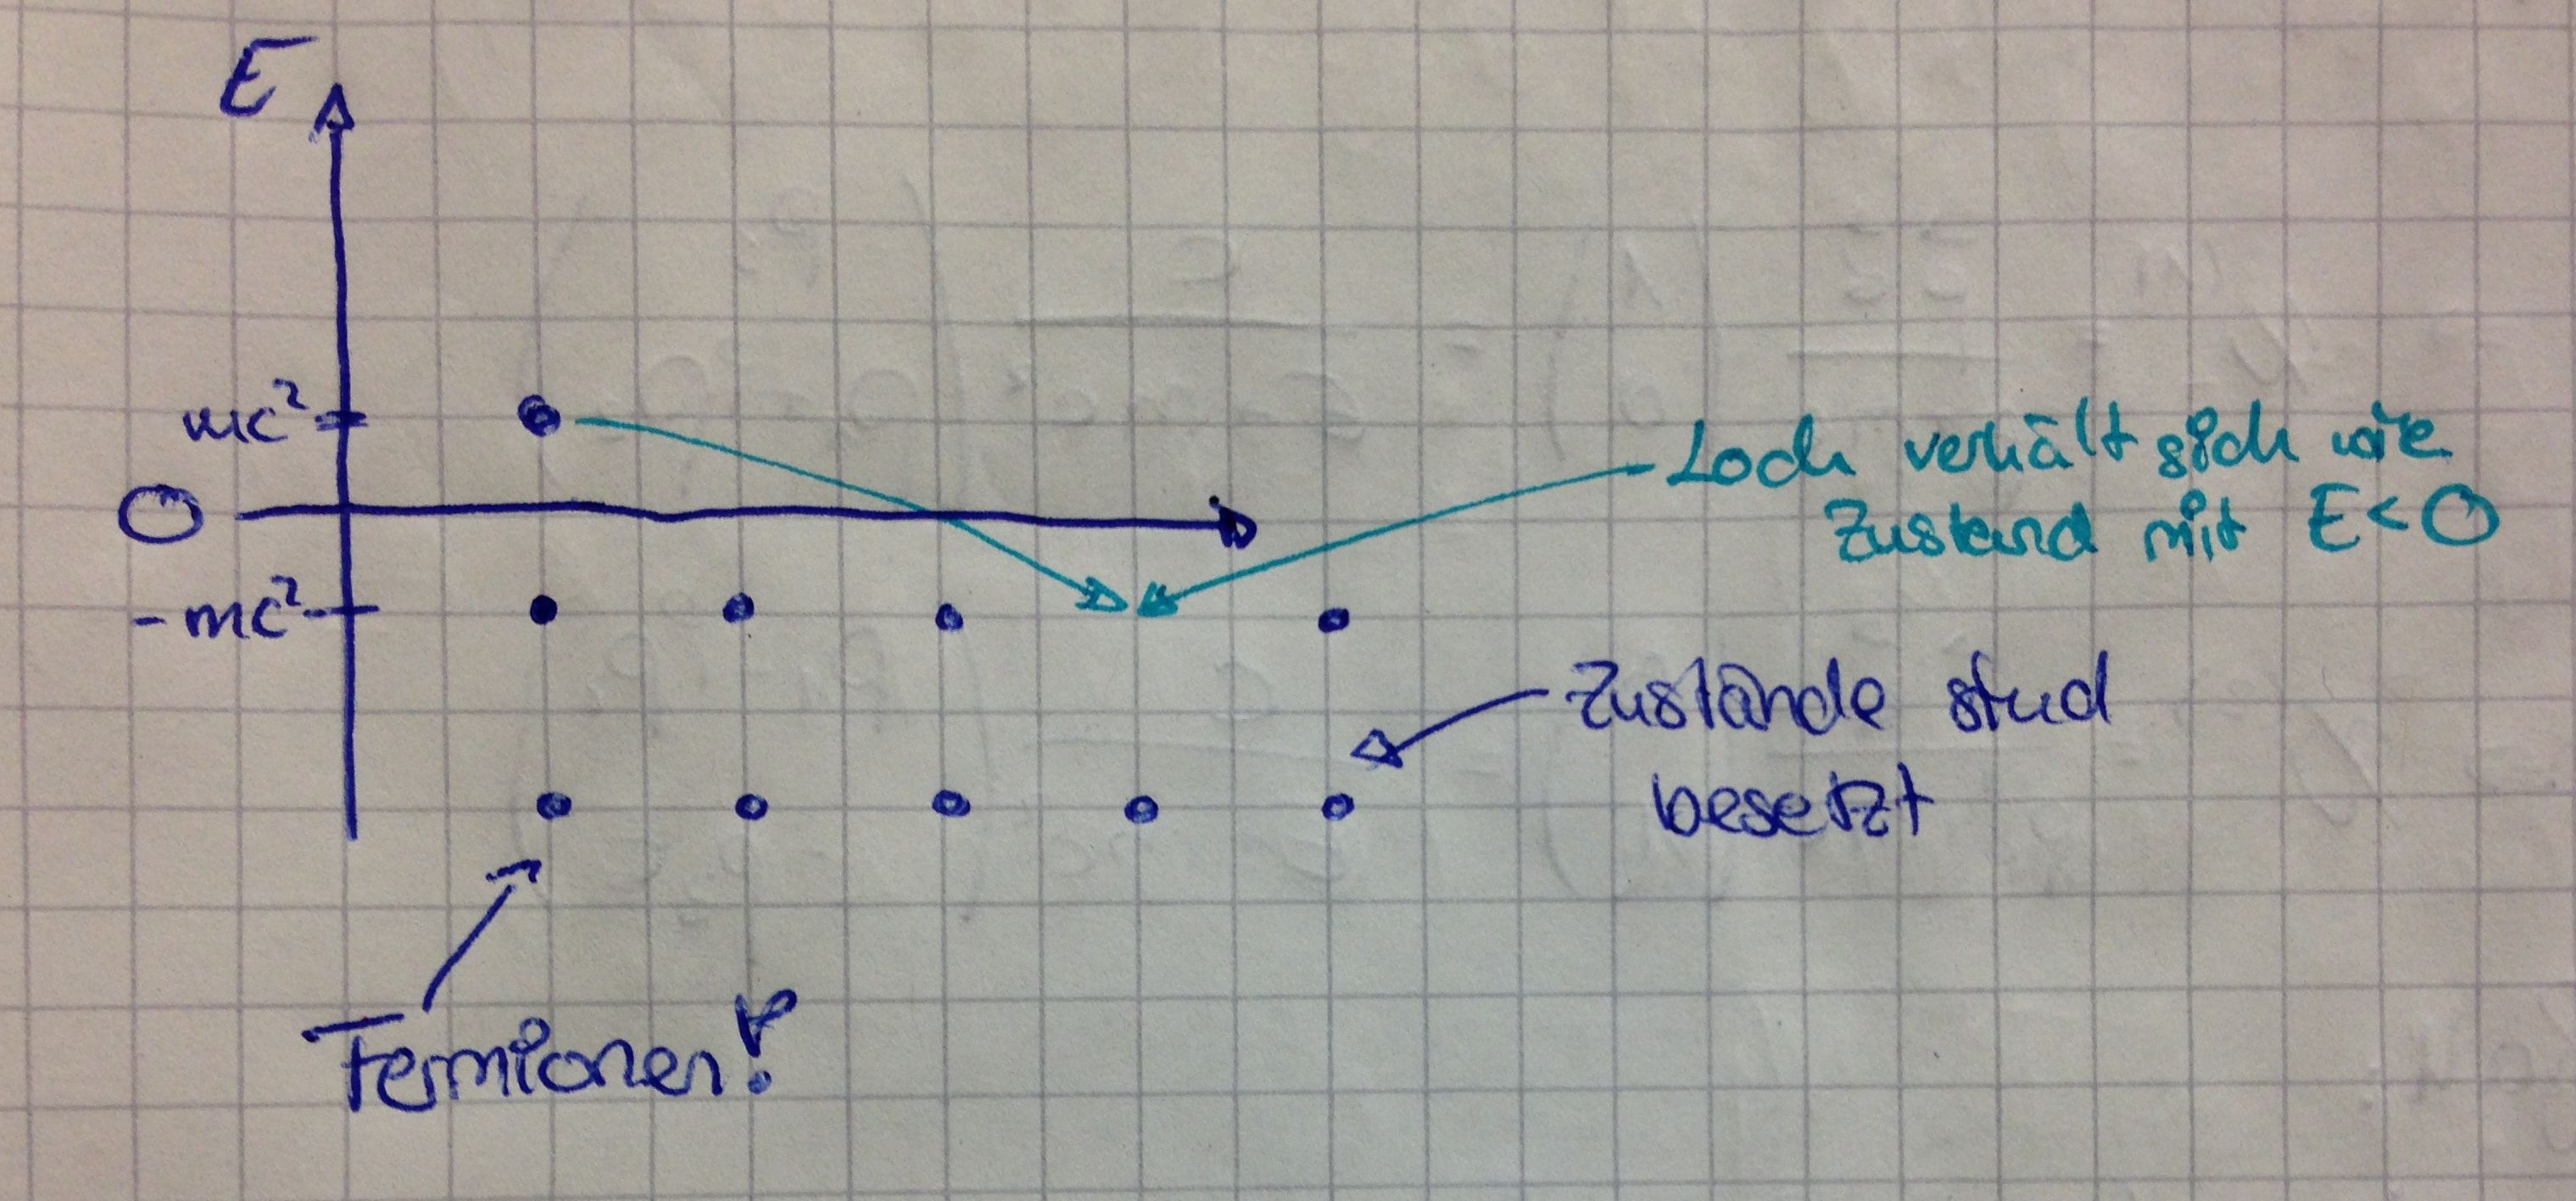
\includegraphics[width=10cm]{Dirac-Gleichung1}
		\end{center}
	\end{figure*}
	
	\\
	\begin{tabular}{l l}
		1928/9 & Vorhersage von Teilchen mit gleicher Masse, aber entgegengesetzter Ladung des Elektrons(Dirac/Weyl) \\
		1932 & Entdeckung des Positrons (Anderson)
	\end{tabular}